\chapter{Results}\label{sec:results}
%correctness - tests done on a set of circuits
%baseline: the original cpu code execution time
%improvements: the mean and the peak speedup
%graphs: speedup vs input size + ESTRAPOLAZIONE
%        speedup vs cell size + ESTRAPOLAZIONE
%speedup prediction accuracy as #cells*2^i/#threads / (real ex. time)
In order to evaluate the performance of CudaQCAD, several tests were executed. These tests aimed to show strengths and fallacies of the simulator both in comparison with the original QCAD and in the usage of the resources offered by the architecture. In the next sections will be described the Hardware used for the tests and the organization of the tests themselves.

\section{Hardware Description}
All the tests were performend using the "Lucifero" Workstation, located in the "MicroLab" of Politecnico di Milano. 

\section{Test 1: CPU vs GPU}
The most meaningful test executed is certainly the comparison between the original QCAD and CudaQCAD. Both the version of the simulator were tested on a pool of QCAs composed by several real circuits of different complexity. This test was designed in order to evaluate:

\begin{description}
\item[Correctness] of the two simulators.
\item[Coherency] of the results.
\item[Performance] in terms of execution time.
\end{description}    

Considering the first two points, the test has shown that both the simulators obtain the same results for all the circuits of the pool and that these results were alligned with the well known behaviour of the circuits.\\
Regarding to the performance, it was noticed a considerable speed-up - 30x of peak - of the GPU version over CPU version only when the number of cells composing the simulated circuits was greater than 7000. For circuits with a lower number of cells, the original QCAD outperform CudaQCAD, Fig x.
 
\begin{figure}[h!bt]
	\centerline{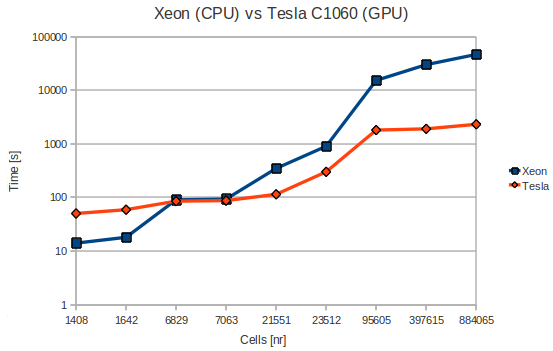
\includegraphics[width=0.7\textwidth]{img/XeonVsTesla.png}}
	\caption{Performance comparison between Intel Xeon and Nvidia Tesla.}
	\label{fig:NvidiaGPUsLogicalOrg}
\end{figure}

This result was not surprising. Until the number of cells in the circuits is lower than a given threshold - 7000 with the used architecture - the overhead due to the memory transfers bertween host and device and the setup times is bigger than the gain due to the parallelism. However, considering that the original goal was to speed-up the simulation of those circuits that requires an amount of time too high to be considered acceptable for pratical purpouses, this test can be considered passed.

\section{Test 2: Memory Transfers}

\section{Test 3: GPU Occupancy}
This test aims to prove the effective usage of the GPU resourcers. The occupancy is the ratio of active warps to the maximum number of warps supported on a multiprocessor of the GPU. As stated in chapter 3, each multiprocessor on the device has a set of N registers available for use by Cuda thread programs. These registers are a shared resource that are allocated among the thread blocks executing on a multiprocessor. The Cuda compiler attempts to minimize register usage to maximize the number of thread blocks that can be active in the machine simultaneously. If a program tries to launch a kernel for which the registers used per thread are too many, the number of threads in concurrent execution will decrease, as consequentely the performance will do.\\
Unfortunalely there is no way to automatic tune the execution parameters in order to achieve the full occupancy. For this reason, several attempts were performed and profiled, Fig X. Considering that the occupancy can be fairy evaluated only when the amout of computations is big enought to require the usages of all the available resources, for this test a circuit with a number of cells greater than the threshold was choosen.\\ 
The first attempt was unsatifactory, due to an occupancy of only 50\%. For this reason the block size was progressively enlarged till achieving the maximum occupancy supported. Unfortunately, even with a larger block size, the occupancy could not be moved to more than 75\%, due to the register pressure.\\
In order to further improve the occupacy, the kernel function was re-designed with special attention to the number of registers per threads, as described in chapter X. The new version of the kernel lead to much better results and the occupation was bring up to 100\%.
    
\begin{figure}[h!bt]
        \centerline{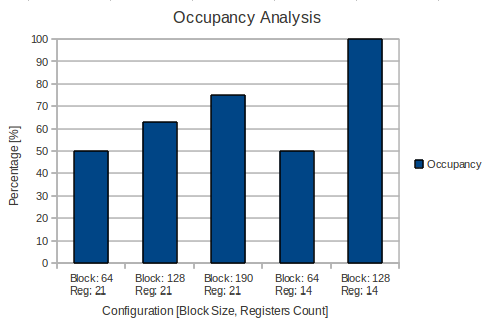
\includegraphics[width=0.7\textwidth]{img/OccupancyAnalysis.png}}
        \caption{Occupancy Analysis. Data extracted from Nvidia Occupancy Calculator.}
        \label{fig:OccupancyAnalysis}
\end{figure}

\section{Test 4: Divergent Branches}
The number of divergent branches can seriously impact on the performance of the simulator. As a rule of thumb the percentage of divergent branches must be lower than 15\% to be considered acceptable. 


